
%%https://ec.gateoverflow.in/1525/gate2020-ec-ga-8
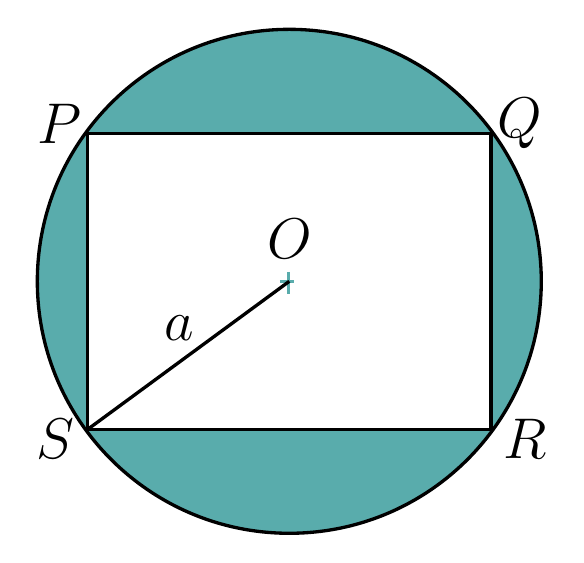
\begin{tikzpicture}[scale = 0.8]
\draw[fill=teal!65!white, very thick](0,0) circle (4);
\draw[fill = white, very thick] (-3.20,-2.35) rectangle (3.20,2.35);
\node[above] at (0,0.2) {\huge{$\text{O}$}};
\node[left] at (-3.15,2.5) {\huge{$\text{P}$}};
\node[left] at (-3.25,-2.5) {\huge{$\text{S}$}};
\node[right] at (3.15,2.5) {\huge{$\text{Q}$}};
\node[right] at (3.25,-2.5) {\huge{$\text{R}$}};
\draw[teal!65!white,very thick] (-0.01,0.15) -- (-0.01,-0.20);
\draw[teal!65!white,very thick] (-0.15,0) -- (0.08,0);
\node[] at (-1.75,-0.75) {\huge{$a$}};
\draw[very thick](-3.20,-2.35) -- (0,0);
\end{tikzpicture}


 %%%%%%%https://gateoverflow.in/313674/gate2017-me-2-ga-10
  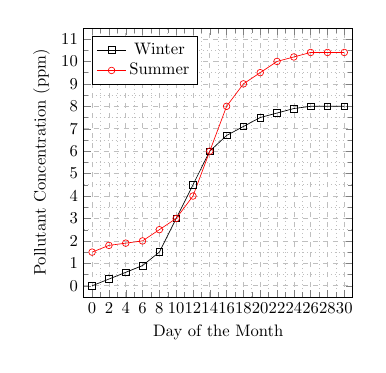
\begin{tikzpicture}[scale=0.6]
\begin{axis}[ylabel=Pollutant Concentration (ppm),xlabel=Day of the Month,
    xtick={0,2,4,6,8,10,12,14,16,18,20,22,24,26,28,30},
    ytick={0,1,2,3,4,5,6,7,8,9,10,11},
    minor tick num=1,
   xmin = -1,xmax=31,ymin=-.5,
    width=0.6\textwidth,
    height=\axisdefaultheight,
    legend pos=north west,
    grid=both,
    grid style={dotted},
    major grid style={dashed},
]
\addplot[black] plot [mark=square] coordinates { (0,0)(2,.3)(4,.6) (6,0.9) (8,1.5)(10,3)(12,4.5)(14,6)(16,6.7)(18,7.1)(20,7.5)(22,7.7)(24,7.9)(26,8)(28,8)(30,8)};
\addplot [red] plot [mark=o] coordinates {(0,1.5)(2,1.8)(4,1.9)(6,2)(8,2.5)(10,3)(12,4)(14,6)(16,8)(18,9)(20,9.5)(22,10)(24,10.2)(26,10.4)(28,10.4)(30,10.4)};
\addlegendentry{Winter}
\addlegendentry{Summer}
\end{axis}
\end{tikzpicture}  


%https://gateoverflow.in/313662/gate2017-me-1-ga-10
       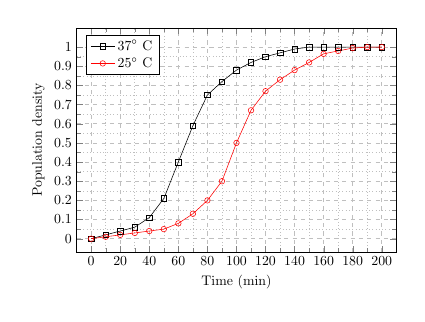
\begin{tikzpicture}[scale=.5]
       
           \begin{axis}[
           ylabel=Population density,
           xlabel=Time (min),
           xtick={0,20,40,60,80,100,120,140,160,180,200},
           ytick={0.0,0.1,0.2,0.3,0.4,0.5,0.6,0.7,0.8,0.9,1.0},
           minor tick num=1,
           xmin = -10,xmax=210,ymin=-0.07,ymax=1.1,
           width=0.8\textwidth,
           height=\axisdefaultheight,
           legend pos=north west,
           grid=both,
           grid style={dotted},
           major grid style={dashed},
        ]
        \addplot[black] plot [mark=square] coordinates {
        (0,0.0) (10,0.02) (20,0.04) (30,0.06) (40,0.11) (50,0.21) (60,0.4) (70,0.59) (80,0.75) (90,0.82) (100,0.88) (110,0.92) (120,0.95) (130,0.97) (140,0.99) (150,1) (160,1) (170,1) (180,1) (190,1) (200,1)};
        \addplot [red] plot [mark=o] coordinates {
        (0,0.0) (10,0.01) (20,0.02) (30,0.03) (40,0.04) (50,0.05) (60,0.08) (70,0.13) (80,0.2) (90,0.3) (100,0.5) (110,0.67) (120,0.77) (130,0.83) (140,0.88) (150,0.92) (160,0.965) (170,0.98) (180,0.995) (190,1.0) (200,1.0)};
        \addlegendentry{37$^{\circ}$ C}
        \addlegendentry{25$^{\circ}$ C}
        \end{axis} 
           
                   
       \end{tikzpicture}


%%https://me.gateoverflow.in/1813/gate-mechanical-2020-set-2-ga-question-10
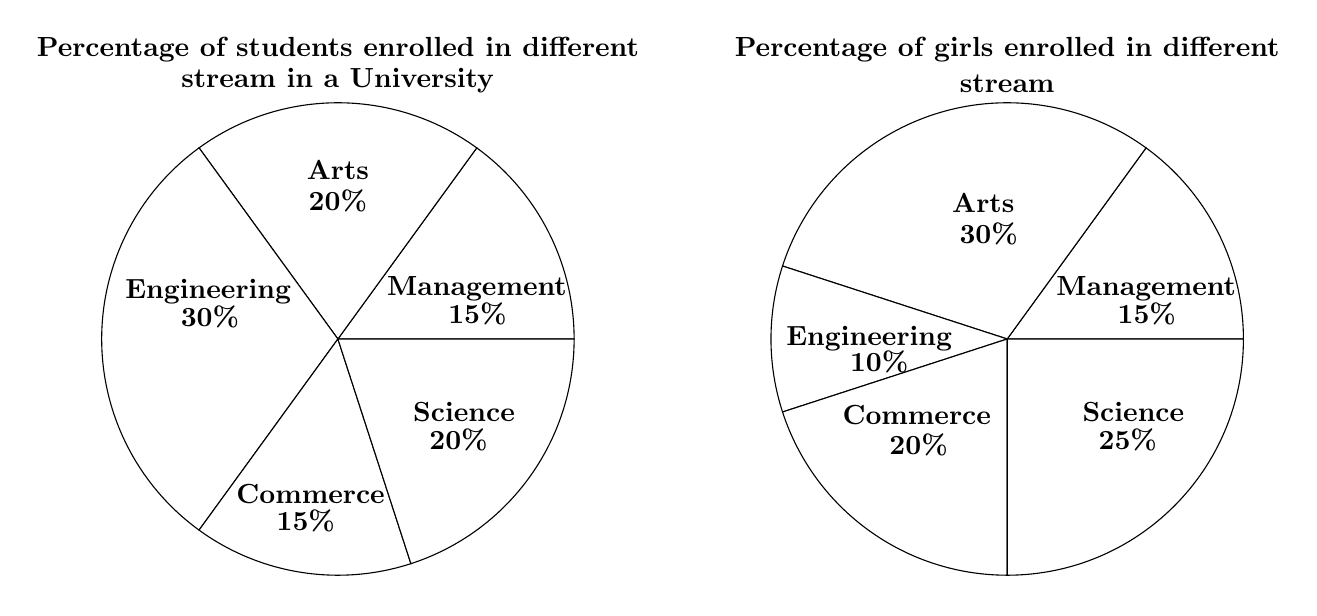
\begin{tikzpicture}
\begin{scope}
\filldraw[draw=black,fill=white] (0,0) -- (0:3cm) arc[start angle=0,end angle=54,radius=3cm] -- cycle;
\filldraw[draw=black,fill=white] (0,0) -- (54:3cm) arc[start angle=54,end angle=126,radius=3cm] -- cycle;
\filldraw[draw=black,fill=white] (0,0) -- (126:3cm) arc[start angle=126,end angle=234,radius=3cm] -- cycle;
\filldraw[draw=black,fill=white] (0,0) -- (234:3cm) arc[start angle=234,end angle=288,radius=3cm] -- cycle;
\filldraw[draw=black,fill=white] (0,0) -- (288:3cm) arc[start angle=288,end angle=360,radius=3cm] -- cycle;

\node[] at (10:1.8cm) {\textbf{15\%}};
\node[] at (20:1.88cm) {\textbf{Management}};

\node[] at (90:1.75cm) {\textbf{20\%}};
\node[] at (90:2.15cm) {\textbf{Arts}};

\node[] at (170:1.65cm) {\textbf{30\%}};
\node[] at (160:1.75cm) {\textbf{Engineering}};

\node[] at (260:2.35cm) {\textbf{15\%}};
\node[] at (260:2cm) {\textbf{Commerce}};

\node[] at (320:2cm) {\textbf{20\%}};
\node[] at (330:1.85cm) {\textbf{Science}};

\node[above] at (0,3.4){\textbf{Percentage of students enrolled in different}};
\node[above] at (0,3) {\textbf{stream in a University}};
\end{scope}

\begin{scope}[xshift = 8.5cm]
\filldraw[draw=black,fill=white] (0,0) -- (0:3cm) arc[start angle=0,end angle=54,radius=3cm] -- cycle;
\filldraw[draw=black,fill=white] (0,0) -- (54:3cm) arc[start angle=54,end angle=162,radius=3cm] -- cycle;
\filldraw[draw=black,fill=white] (0,0) -- (162:3cm) arc[start angle=162,end angle=198,radius=3cm] -- cycle;
\filldraw[draw=black,fill=white] (0,0) -- (198:3cm) arc[start angle=198,end angle=270,radius=3cm] -- cycle;
\filldraw[draw=black,fill=white] (0,0) -- (270:3cm) arc[start angle=270,end angle=360,radius=3cm] -- cycle;

\node[] at (10:1.8cm) {\textbf{15\%}};
\node[] at (20:1.88cm) {\textbf{Management}};

\node[] at (100:1.35cm) {\textbf{30\%}};
\node[] at (100:1.75cm) {\textbf{Arts}};

\node[] at (190:1.65cm) {\textbf{10\%}};
\node[] at (180:1.75cm) {\textbf{Engineering}};

\node[] at (230:1.75cm) {\textbf{20\%}};
\node[] at (220:1.5cm) {\textbf{Commerce}};

\node[] at (320:2cm) {\textbf{25\%}};
\node[] at (330:1.85cm) {\textbf{Science}};

\node[above] at (0,3.4){\textbf{Percentage of girls enrolled in different}};
\node[above] at (0,3) {\textbf{stream}};
\end{scope}
\end{tikzpicture}

%%https://ch.gateoverflow.in/1156/gate-chemical-2020-ga-question-10
%%https://gateoverflow.in/359808/gate-chemical-2020-ga-question-10
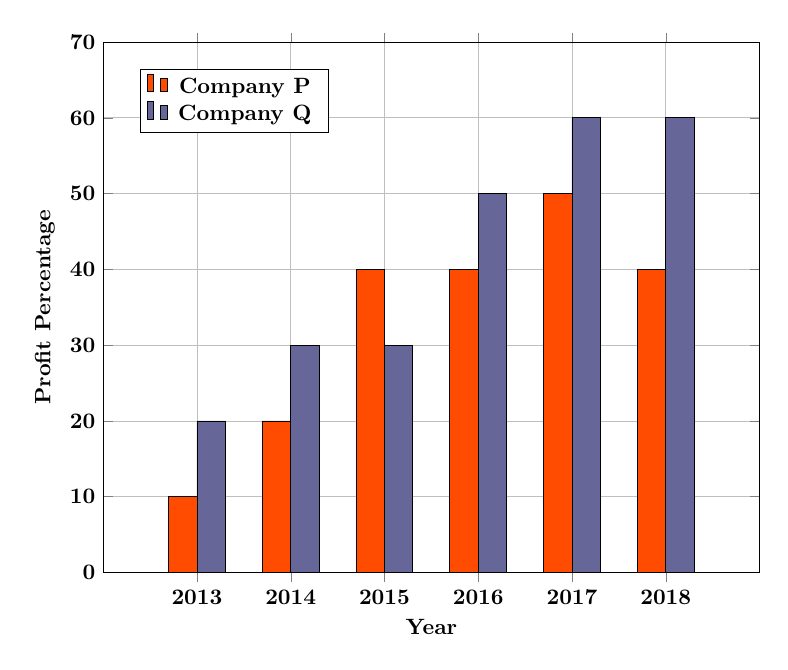
\begin{tikzpicture}[scale = 0.8,font = \bfseries]
\begin{axis}[
ybar=0pt, %space between adjacent bars is 0
enlarge x limits=0.20,
enlarge y limits=false,
legend style={at={(0.20,0.95),ybar=area},
anchor=north,legend columns=1.5},
ylabel= Profit Percentage,
xlabel= Year,
ymajorgrids = true,
xmajorgrids = true,
symbolic x coords={2013,2014,2015,2016,2017,2018},
xtick=data,
ytick={0,10,20,...,80},
bar width=0.45cm,
%style={font=\boldmath},
nodes near coords align={vertical},
%every x tick label/.append style={font=\bfseries},
every y tick label/.append style={font=\boldmath},
%tick label style={font=\boldmath}, 
label style={color=black,font=\bfseries},
width=12cm,
height=10cm,
ymax=70,
ymin=0
]
\addplot
[fill=red!40!orange,draw=black,mark=none]
coordinates {(2013,10) (2014,20) (2015,40) (2016,40) (2017,50) (2018,40)};
\addplot
[fill=blue!20!gray,draw=black]
coordinates {(2013,20) (2014,30) (2015,30) (2016,50) (2017,60) (2018,60)};
\legend{\;Company P\;,Company Q}

\end{axis}
\end{tikzpicture}




%%https://gateoverflow.in/359518/gate-mechanical-2020-set-1-ga-question-10
%%https://me.gateoverflow.in/1711/gate-mechanical-2020-set-1-ga-question-10

\begin{tikzpicture}[scale = 0.8,font = \bfseries]
\begin{axis}[
ybar=0pt, %space between adjacent bars is 0
enlarge x limits=0.18,
enlarge y limits=false,
title={Performance of Schools P, Q, R and S},
legend style={at={(0.18,0.97),ybar=area},
anchor=north,legend columns=-1},
ylabel= {Number of students},
symbolic x coords={School P, School Q, School R, School S},
xtick=data,
ytick={0,100,200,...,800,900,1000},
nodes near coords,
bar width=0.75cm,
ymajorgrids = true,
every node near coord/.append style={font=\boldmath},
nodes near coords align={vertical},
every x tick label/.append style={font=\bfseries},
every y tick label/.append style={font=\boldmath},
%tick label style={font=\boldmath}, 
label style={color=black,font=\bfseries},
width=14cm,
height=10cm,
ymax=800,
ymin=0
]
\addplot
[fill=magenta!40!white,postaction={
        pattern=north west lines
    },draw=black]
coordinates {(School P,500) (School Q,600) (School R,700) (School S,400)};
\addplot
[fill=blue!40!white,postaction={
        pattern=north east lines
    },draw=black]
coordinates {(School P,280) (School Q,330) (School R,455) (School S,240)};
\legend{Appeared\;\;,Passed}
\end{axis}
\end{tikzpicture}


%%https://gateoverflow.in/359759/gate-ece-2020-ga-question-10
%%https://ec.gateoverflow.in/1523/gate-ece-2020-ga-question-10

\begin{tikzpicture}[scale = 0.8,font = \bfseries]
\begin{axis}[
ybar=0pt, %space between adjacent bars is 0
enlarge x limits=0.20,
enlarge y limits=false,
legend style={at={(0.18,0.97),ybar=area},
anchor=north,legend columns=1},
ylabel= Number of students (in thousands),
xlabel= Year,
ymajorgrids = true,
xmajorgrids = true,
symbolic x coords={2014,2015,2016,2017,2018},
xtick=data,
ytick={0,1,2,...,8,9,10},
bar width=0.5cm,
every node near coord/.append style={font=\boldmath},
nodes near coords align={vertical},
every x tick label/.append style={font=\bfseries},
every y tick label/.append style={font=\boldmath},
%tick label style={font=\boldmath}, 
label style={color=black,font=\bfseries},
width=12cm,
height=10cm,
ymax=9,
ymin=0
]
\addplot
[fill=red!40!orange,postaction={
        pattern=north east lines
    },draw=black]
coordinates {(2014,3) (2015,5) (2016,5) (2017,6) (2018,4)};
\addplot
[fill=blue!20!gray,postaction={
        pattern= vertical lines
    }, draw=black]
coordinates {(2014,4) (2015,7) (2016,8) (2017,7) (2018,5)};
\legend{\;School P\;,School Q}

\end{axis}
\end{tikzpicture}



%%https://gateoverflow.in/359710/gate-electrical-2020-ga-question-10
%%https://ee.gateoverflow.in/1483/gate-electrical-2020-ga-question-10

\begin{tikzpicture}[scale = 0.8,font = \bfseries]
\begin{axis}[
ybar=0pt, %space between adjacent bars is 0
enlarge x limits=0.20,
enlarge y limits=false,
title={Revenue and Expenditure (in million rupees) of four  \\ companies P, Q, R and S in 2015},
title style={yshift=1mm,align=center},
legend style={at={(0.5,0.97),ybar=area},
anchor=north,legend columns=-1},
ylabel= Revenue/Expenditure (in million rupees),
symbolic x coords={Company P, Company Q, Company R, Company S},
xtick=data,
ytick={0,5,10,...,50,55,60},
bar width=0.60cm,
ymajorgrids = true,
every node near coord/.append style={font=\boldmath},
nodes near coords align={vertical},
every x tick label/.append style={font=\bfseries},
every y tick label/.append style={font=\boldmath},
%tick label style={font=\boldmath}, 
label style={color=black,font=\bfseries},
width=12cm,
height=10cm,
ymax=55,
ymin=0
]
\addplot
[fill=magenta!40!white,postaction={
        pattern=north west lines
    },draw=black]
coordinates {(Company P,35) (Company Q,45) (Company R,30) (Company S,40)};
\addplot
[fill=blue!40!white,postaction={
        pattern=north east lines
    },draw=black]
coordinates {(Company P,25) (Company Q,35) (Company R,40) (Company S,50)};
\legend{Revenue\;\;,Expenditure}
\end{axis}
\end{tikzpicture}

%https://gateoverflow.in/313419/gate2017-ce-2-ga-10
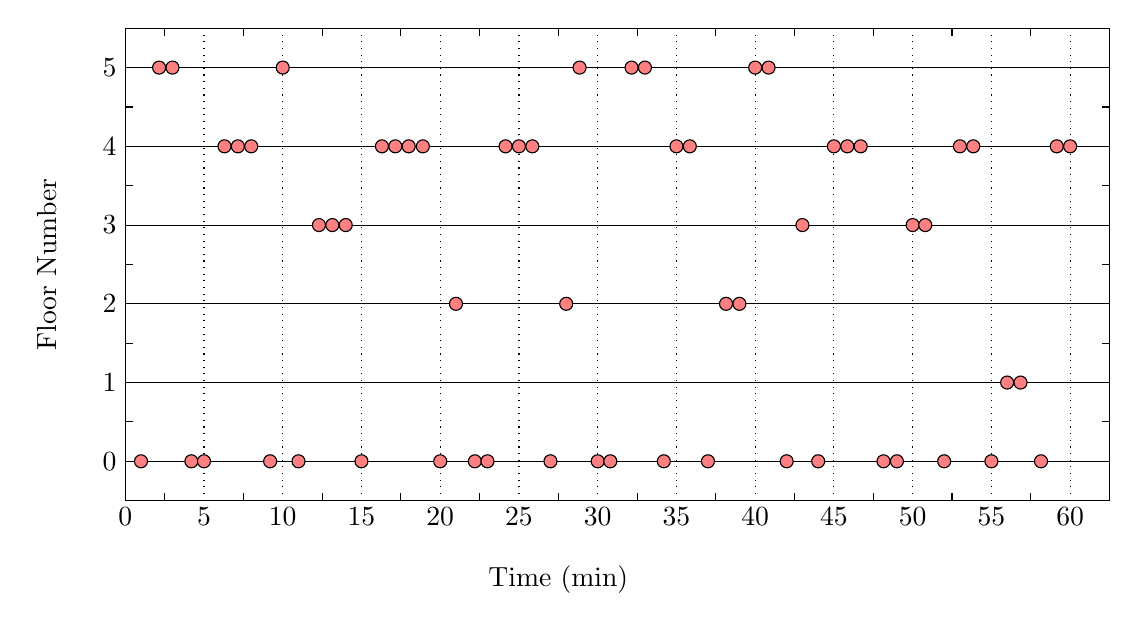
\begin{tikzpicture}
            \tikzstyle{nodep}=[circle,draw,scale=.5,fill=red!50]
            
            \draw[-] (0,6)--(12.5,6)--(12.5,0)--(0,0)--(0,6); 
    
             \draw (0,-.2) node {0};
             \draw (1,-.2) node {5};
             \draw (2,-.2) node {10};
             \draw (3,-.2) node {15};
             \draw (4,-.2) node {20};
             \draw (5,-.2) node {25};
             \draw (6,-.2) node {30};
             \draw (7,-.2) node {35};
             \draw (8,-.2) node {40};
             \draw (9,-.2) node {45};
             \draw (10,-.2) node {50};
             \draw (11,-.2) node {55};
             \draw (12,-.2) node {60};
             
            \foreach \x in {1,2,...,12}
            {
                \draw[dotted] (\x,0)--(\x,6);
            }
            \foreach \x in {.5,1.5,...,11.5}
            {
                \draw[-] (\x,0)--(\x,.1);
            }
            \foreach \x in {.5,1.5,...,11.5}
            {
                \draw[-] (\x,6)--(\x,5.9);
            
            }
            \draw (-.2,.5) node {0};
            \draw (-.2,1.5) node {1};
            \draw (-.2,2.5) node {2};
            \draw (-.2,3.5) node {3};
            \draw (-.2,4.5) node {4};
            \draw (-.2,5.5) node {5};
            
             \foreach \y in {.5,...,5.5}
            {
                \draw[-] (0,\y)--(12.5,\y);
            }
             \foreach \y in {1,...,5}
            {
                \draw[-] (0,\y)--(.1,\y);
            }
             \foreach \y in {1,...,5}
            {
                \draw[-] (12.5,\y)--(12.4,\y);
            }
            
            %ground_floor
            \node[nodep] at (.2,.5) {};
            \node[nodep] at (.84,.5) {};
            \node[nodep] at (1,.5) {};
            \node[nodep] at (1.84,.5) {};
            \node[nodep] at (2.2,.5) {};
            \node[nodep] at (3,.5) {};
            \node[nodep] at (4,.5) {};
            \node[nodep] at (4.44,.5) {};
            \node[nodep] at (4.6,.5) {};
            \node[nodep] at (5.4,.5) {};
            \node[nodep] at (6,.5) {};
            \node[nodep] at (6.16,.5) {};
            \node[nodep] at (6.84,.5) {};
            \node[nodep] at (7.4,.5) {};
            \node[nodep] at (8.4,.5) {};
            \node[nodep] at (8.8,.5) {};
            \node[nodep] at (9.63,.5) {};
            \node[nodep] at (9.8,.5) {};
            \node[nodep] at (10.4,.5) {};
            \node[nodep] at (11,.5) {};
            \node[nodep] at (11.63,.5) {};
            
            %first_floor
            \node[nodep] at (11.2,1.5) {};
            \node[nodep] at (11.37,1.5) {};
            
            %second_floor
            \node[nodep] at (4.2,2.5) {};
            \node[nodep] at (5.6,2.5) {};
            \node[nodep] at (7.63,2.5) {};
            \node[nodep] at (7.8,2.5) {};
            
            %third_floor
            \node[nodep] at (2.46,3.5) {};
            \node[nodep] at (2.63,3.5) {};
            \node[nodep] at (2.8,3.5) {};
            \node[nodep] at (8.6,3.5) {};
            \node[nodep] at (10,3.5) {};
            \node[nodep] at (10.16,3.5) {};
            
            %fourth_floor
            \node[nodep] at (1.26,4.5) {};
            \node[nodep] at (1.43,4.5) {};
            \node[nodep] at (1.6,4.5) {};
            \node[nodep] at (3.26,4.5) {};
            \node[nodep] at (3.43,4.5) {};
            \node[nodep] at (3.6,4.5) {};
            \node[nodep] at (3.78,4.5) {};
            \node[nodep] at (4.83,4.5) {};
            \node[nodep] at (5,4.5) {};
            \node[nodep] at (5.17,4.5) {};
            \node[nodep] at (7,4.5) {};
            \node[nodep] at (7.17,4.5) {};
            \node[nodep] at (9,4.5) {};
            \node[nodep] at (9.17,4.5) {};
            \node[nodep] at (9.34,4.5) {};
            \node[nodep] at (10.6,4.5) {};
            \node[nodep] at (10.77,4.5) {};
            \node[nodep] at (11.83,4.5) {};
            \node[nodep] at (12,4.5) {};
            
            %fifth_floor
            \node[nodep] at (.43,5.5) {};
            \node[nodep] at (.6,5.5) {};
            \node[nodep] at (2,5.5) {};
            \node[nodep] at (5.77,5.5) {};
            \node[nodep] at (6.43,5.5) {};
            \node[nodep] at (6.6,5.5) {};
            \node[nodep] at (8,5.5) {};
            \node[nodep] at (8.17,5.5) {};
            
            \draw (-1,3) node[rotate=90] {Floor Number};
            \draw (5.5,-1) node {Time (min)};
            
       \end{tikzpicture}







%% https://me.gateoverflow.in/1818/gate2020-me-2-ga-5

\begin{tikzpicture}[transform shape,scale = 0.8]
\draw[thick,rounded corners] (0,0) rectangle (2,1);
\draw[thick,rounded corners] (3,0) rectangle (5,1);
\draw[thick,rounded corners] (6,0) rectangle (8,1);
\draw[thick,rounded corners] (9,0) rectangle (11,1);
\draw[thick,rounded corners] (12,0) rectangle (14,1);
\draw[thick,rounded corners] (15,0) rectangle (17,1);
\node[left] at (1.25,0.5){$\text{P}$};
\node[left] at (4.25,0.5){$\text{Q}$};
\node[left] at (7.25,0.5){$\text{R}$};
\node[left] at (10.25,0.5){$\text{S}$};
\node[left] at (13.25,0.5){$\text{T}$};
\node[left] at (16.90,0.5){$\text{Customers}$};
\draw[-{Triangle[width=14pt,length=6pt,]}, line width=6pt,gray!65!white](2.20,0.5) -- (2.80, 0.5);
\draw[-{Triangle[width=14pt,length=6pt,]}, line width=6pt,gray!65!white](5.20,0.5) -- (5.80, 0.5);
\draw[-{Triangle[width=14pt,length=6pt,]}, line width=6pt,gray!65!white](8.20,0.5) -- (8.80, 0.5);
\draw[-{Triangle[width=14pt,length=6pt,]}, line width=6pt,gray!65!white](11.20,0.5) -- (11.80, 0.5);
\draw[-{Triangle[width=14pt,length=6pt,]}, line width=6pt,gray!65!white](14.20,0.5) -- (14.80, 0.5);
\end{tikzpicture}


%%https://gateoverflow.in/333232/gate-cse-2020-question-ga-9

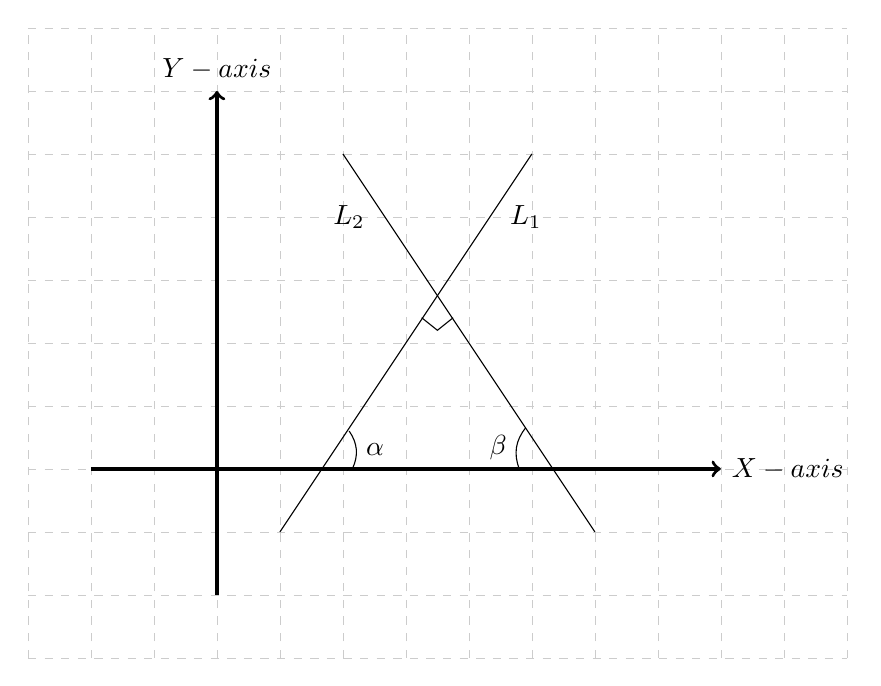
\begin{tikzpicture}[scale = 0.8]
\draw[help lines, color=gray!40, dashed] (-3,-3) grid (10,7);
\draw[->,very thick] (-2,0)--(8,0) node[right]{$\text{X-axis}$};
\draw[->,very thick] (0,-2)--(0,6) node[above]{$\text{Y-axis}$};
\draw [] (1,-1) -- (5,5);
\draw [] (6,-1) -- (2,5);
\path[right](2.10,0.60)  edge  [bend left]  node {$\alpha$} (2.15,0);
\path[left](4.90,0.65)  edge  [bend right]  node {$\beta$} (4.80,0);
\draw[] (3.25,2.40) -- (3.5,2.20) -- (3.75,2.40);
\node[right] at (4.5,4) {$L_{1}$};
\node[left] at (2.5,4) {$L_{2}$};
\end{tikzpicture}



%https://ee.gateoverflow.in/1484/gate2020-ee-ga-9

\begin{tikzpicture}
\node at (0.0,1.7) {C};
\node at (0.0,-1.4) {O};
\node at (-2.5,-0.9) {A};
\node at (2.5,-0.9) {B};
\node [draw , semicircle, minimum size= 2.2cm, line width=0.5mm] at (0.0,0.0) {};
\draw[-] (0.0,-0.9) -- (0.0,1.3);
\draw[-, color =blue, line width=0.5mm] (-2.2,-0.9) -- (0.0,1.3);
\draw[-, color =blue, line width=0.5mm] (2.2,-0.9) -- (0.0,1.3);
\draw[-] (0.2,-0.9) -- (0.2,-0.7);
\draw[-] (0.0,-0.7) -- (0.2,-0.7);
\end{tikzpicture}



%https://me.gateoverflow.in/1814/gate2020-me-2-ga-9

\begin{tikzpicture}[>=stealth',shorten >=1pt,auto,thick,node distance=2.8cm]
\node at (-0.1,1.9) {\text{\small{(X,Y)}}};
\node at (2.4,-0.3) {\text{\small{Z}}};
\node at (0.1,-0.2) {\text{\small{O}}};

\draw[->,line width=0.4mm] (0.0,0.0) -- (2.5,0.0);
\draw[->,line width=0.4mm] (0.4,-0.4) -- (0.4,2.5);
\draw[-, color=blue,line width=0.4mm] (0.4,0.0) -- (1.2,2.1);
\end{tikzpicture}



%%https://gateoverflow.in/333233/gate-cse-2020-question-ga-8

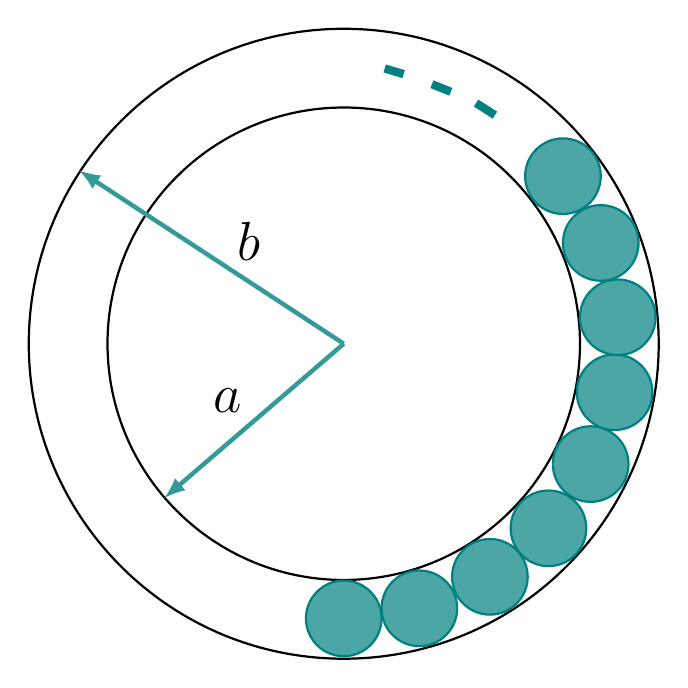
\begin{tikzpicture}[scale = 0.8,transform shape]
\draw[thick](0,0) circle (5);
\draw[thick](0,0) circle (3.75);
\draw[fill=teal!70!white,draw=teal,thick](0,-4.36) circle (0.60);
\draw[fill=teal!70!white,draw=teal,thick](1.20,-4.20) circle (0.60);
\draw[fill=teal!70!white,draw=teal,thick](2.32,-3.70) circle (0.60);
\draw[fill=teal!70!white,draw=teal,thick](3.25,-2.93) circle (0.60);
\draw[fill=teal!70!white,draw=teal,thick](3.92,-1.91) circle (0.60);
\draw[fill=teal!70!white,draw=teal,thick](4.30,-0.77) circle (0.60);
\draw[fill=teal!70!white,draw=teal,thick](4.35,0.42) circle (0.60);
\draw[fill=teal!70!white,draw=teal,thick](4.08,1.60) circle (0.60);
\draw[fill=teal!70!white,draw=teal,thick](3.48,2.66) circle (0.60);

\draw[draw=teal, ultra thick,line width=3pt] (2.10,3.82) -- (2.40,3.63);
\draw[draw=teal, ultra thick,line width=3pt] (1.40,4.12) -- (1.70,4);
\draw[draw=teal, ultra thick, line width=3pt] (0.65,4.37) -- (0.95,4.28);

\draw[->,>=latex, ultra thick,teal!80!white] (0,0) -- (-4.20,2.75);
\draw[->,>=latex,ultra thick,teal!80!white] (0,0) -- (-2.85,-2.45);

\node[above] at (-1.5,1.20) {\Huge{$b$}};
\node[left] at (-1.5,-0.90) {\Huge{$a$}};
\end{tikzpicture}







%%https://gateoverflow.in/333231/gate-cse-2020-question-ga-10
\definecolor{mintbg}{rgb}{.63,.79,.95}

    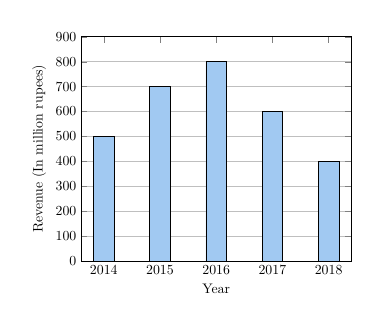
\begin{tikzpicture}[scale= 0.5,transform shape]
        \begin{axis}[
        ybar stacked,
        ymin=0,
        ymax=900,
        ytick={0,100,...,900},
            symbolic x coords={2014,2015,2016,2017,2018},
           xtick=data,
             ylabel near ticks,
    xlabel near ticks,
              xlabel={Year},
              ymajorgrids = true,
   ylabel={Revenue (In million rupees)} ]
            \addplot[ybar,fill=mintbg,bar width=15pt] coordinates {
                (2014, 500)
                (2015, 700)
                (2016, 800)
                (2017, 600)
                (2018, 400)
               
            };
        \end{axis}
    \end{tikzpicture}








%%https://me.gateoverflow.in/1712/gate-mechanical-2020-set-1-ga-question-9
%answer image
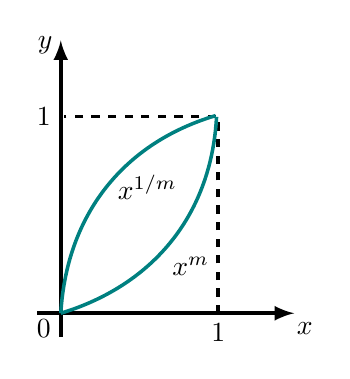
\begin{tikzpicture}[>=latex,shorten >=1pt,auto, semithick,node distance=2.8cm,scale = 1]
\node[] at (-0.2,3.4) {$y$};
\node[left] at (0,2.5) {$1$};
\node[left] at (0,-0.2) {$0$};
\node[below] at (2.0,0) {$1$};
\node[] at (3.1,-0.2) {$x$};
\node[] at (1.65,0.6) {$x^{m}$};
\node[] at (1.1,1.6) {$x^{1/m}$};
\draw[->,line width=0.5mm] (0.0,-0.3) -- (0.0,3.5);
\draw[->,line width=0.5mm] (-0.3,0.0) -- (3.0,0.0);
\draw[-,line width=0.45mm,dashed](2.0,0.0) -- (2.0,2.5) -- (0.0,2.5);
\path[-,line width=0.45mm]
[teal] (0.0,0.0) edge [bend left = 35]  node  {} (2.0,2.52)
[teal] (0.0,0.0) edge [bend right = 35]  node  {} (1.98,2.53);
\end{tikzpicture}

%%https://ch.gateoverflow.in/1159/gate-chemical-2020-ga-question-7
%answer image 1
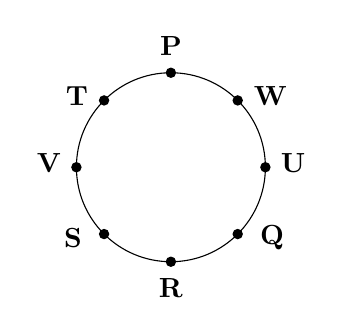
\begin{tikzpicture}[scale = 0.6]
    % equidistant points and arc
    \foreach \x [count=\p] in {0,...,7} {
        \node[shape=circle,fill=black, scale=0.4] (\p) at (-\x*45:2) {};};
    \draw (1) arc (0:360:2);

\node[above] at (0,2.15) {$\textbf{P}$};    
\node[below] at (0,-2.15) {$\textbf{R}$}; 
\node[right] at (1.55,1.5) {$\textbf{W}$};    
\node[left] at (-1.55,1.5) {$\textbf{T}$}; 
\node[right] at (2.12,0.08) {$\textbf{U}$};   
\node[left] at (-2.12,0.08) {$\textbf{V}$};   
\node[right] at (1.68,-1.5) {$\textbf{Q}$};  
\node[left] at (-1.68,-1.5) {$\textbf{S}$}; 

\end{tikzpicture}
%answer image 2
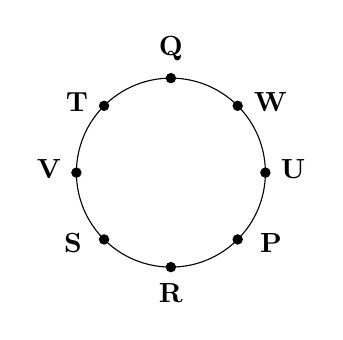
\begin{tikzpicture}[scale = 0.6]
    % equidistant points and arc
    \foreach \x [count=\p] in {0,...,7} {
        \node[shape=circle,fill=black, scale=0.4] (\p) at (-\x*45:2) {};};
    \draw (1) arc (0:360:2);

\node[above] at (0,2.15) {$\textbf{Q}$};    
\node[below] at (0,-2.15) {$\textbf{R}$}; 
\node[right] at (1.55,1.5) {$\textbf{W}$};    
\node[left] at (-1.55,1.5) {$\textbf{T}$}; 
\node[right] at (2.12,0.08) {$\textbf{U}$};   
\node[left] at (-2.12,0.08) {$\textbf{V}$};   
\node[right] at (1.68,-1.5) {$\textbf{P}$};  
\node[left] at (-1.68,-1.5) {$\textbf{S}$}; 
\end{tikzpicture}


%%https://me.gateoverflow.in/1816/gate2020-me-2-ga-7
%question-image
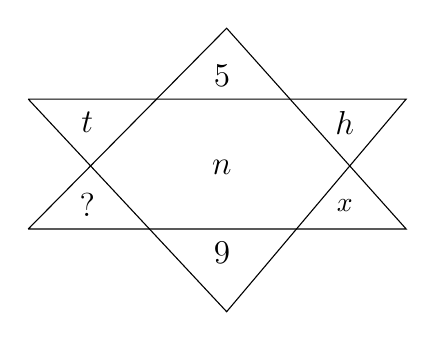
\begin{tikzpicture}[scale = 0.6]
\draw[] (0,0) -- (8,0) -- (4.20,-4.5) -- (0,0);
\draw[] (0,-2.75) -- (8,-2.75) -- (4.20,1.5) -- (0,-2.75);
\node[] at (4.1,0.5){\large{$5$}};
\node[] at (4.1,-3.25){\large{$9$}};
\node[] at (1.25,-0.5){\large{$t$}};
\node[] at (1.25,-2.25){\large{$?$}};
\node[] at (6.70,-0.5){\large{$h$}};
\node[] at (6.70,-2.25){$x$};
\node[] at (4.1,-1.45){\large{$n$}};
\end{tikzpicture}
%%https://me.gateoverflow.in/1816/gate2020-me-2-ga-7
%answer-image1
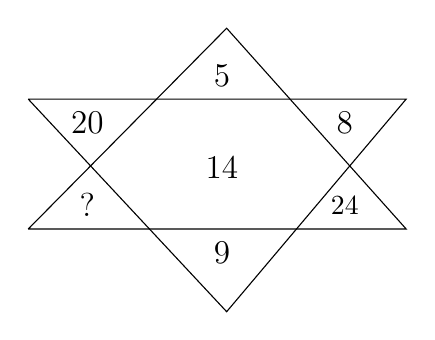
\begin{tikzpicture}[scale = 0.6]
\draw[] (0,0) -- (8,0) -- (4.20,-4.5) -- (0,0);
\draw[] (0,-2.75) -- (8,-2.75) -- (4.20,1.5) -- (0,-2.75);
\node[] at (4.1,0.5){\large{$5$}};
\node[] at (4.1,-3.25){\large{$9$}};
\node[] at (1.25,-0.5){\large{$20$}};
\node[] at (1.25,-2.25){\large{$?$}};
\node[] at (6.70,-0.5){\large{$8$}};
\node[] at (6.70,-2.25){$24$};
\node[] at (4.1,-1.45){\large{$14$}};
\end{tikzpicture}
%%https://me.gateoverflow.in/1816/gate2020-me-2-ga-7
%answer-image2
\begin{tikzpicture}[node distance=25mm,auto,scale = 0.8]
\node[state,minimum size= 0.5mm] (q0) {$14$};
\node[state,minimum size= 0.5mm] (q1)[above of  = q0] {$5$};
\node[state,minimum size= 0.5mm] (q2)[below of  = q0] {$9$};
\node[state,minimum size= 0.5mm] at (-3,1.25) (q3) {$20$};
\node[state,minimum size= 0.5mm] at (-3,-1.25)(q4) {$4$};
\node[state,minimum size= 0.5mm] at (3,1.25)(q5) {$8$};
\node[state,minimum size= 0.5mm] at (3,-1.25)(q6) {$24$};
\path[] (q0) edge[above left,pos = 0.90,sloped] node {$14-9$} (q1);
\path[] (q0) edge[below right,pos = 0.90,sloped,rotate=180] node {$14-5$} (q2);
\path[] (q0) edge[above right,pos = 0.85,sloped] node {$14+6$} (q3);
\path[] (q0) edge[above right,pos = 0.85,sloped] node {$14-10$} (q4);
\path[] (q0) edge[above right,pos = 0.25,sloped] node {$14-6$} (q5);
\path[] (q0) edge[above right,pos = 0.25,sloped] node {$14+10$} (q6);
\end{tikzpicture}



%%https://civil.gateoverflow.in/1668/gate2020-ce-1-ga-10
%question image
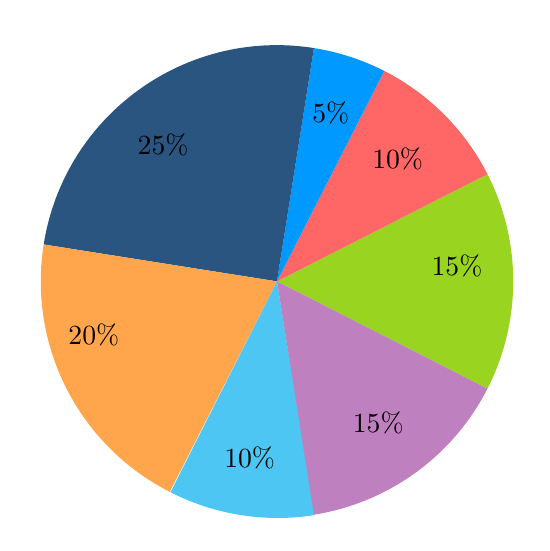
\begin{tikzpicture}
\tikzset{
     lines/.style={draw=none},
}
\pie[text = legend,style={lines},color={blue!40!cyan,red!60!white, yellow!60!green, violet!50!white,cyan!70!white,orange!70!white,{rgb:red,1;green,2;blue,3}}]
{5/Health (5\%),
 10/Transport (10\%),
 15/Household Items (15\%),
 15/Education (15\%),
 10/Leisure (10\%),
 20/House rent (20\%),
 25/Others (25\%)
 }
\filldraw[draw=none,fill=yellow!60!green] (0,0) -- (-27:3cm) arc[start angle=-27,end angle=27,radius=3cm] -- cycle;
\filldraw[draw=none,fill=red!60!white] (0,0) -- (27:3cm) arc[start angle=27,end angle=63,radius=3cm] -- cycle;
\filldraw[draw=none,fill=blue!40!cyan] (0,0) -- (63:3cm) arc[start angle=63,end angle=81,radius=3cm] -- cycle;
\filldraw[draw=none,fill={rgb:red,1;green,2;blue,3}] (0,0) -- (81:3cm) arc[start angle=81,end angle=171,radius=3cm] -- cycle;
\filldraw[draw=none,fill=orange!70!white] (0,0) -- (171:3cm) arc[start angle=171,end angle=243,radius=3cm] -- cycle;
\filldraw[draw=none,fill=cyan!70!white] (0,0) -- (243.2:3cm) arc[start angle=243,end angle=279,radius=3cm] -- cycle;
\filldraw[draw=none,fill=violet!50!white] (0,0) -- (279:3cm) arc[start angle=279,end angle=333,radius=3cm] -- cycle;

\node[right] at (6:1.85cm) {\text{15\%}};

\node[above] at (40:2cm) {\text{10\%}};

\node[above] at (70:2cm) {\text{5\%}};

\node[left] at (120:2cm) {\text{25\%}};

\node[left] at (200:2cm) {\text{20\%}};

\node[below] at (260:2cm) {\text{10\%}};

\node[below] at (310:2cm) {\text{15\%}};


\end{tikzpicture}


%https://me.gateoverflow.in/1712/gate2020-me-1-ga-9
%answer image 1
 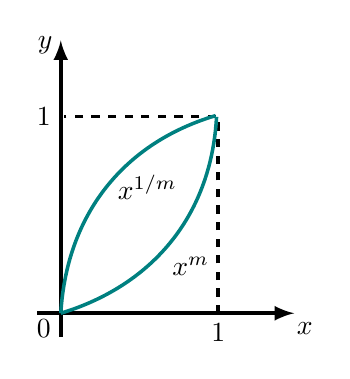
\begin{tikzpicture}[>=latex,shorten >=1pt,auto, semithick,node distance=2.8cm,scale = 1]
\node[] at (-0.2,3.4) {$y$};
\node[left] at (0,2.5) {$1$};
\node[left] at (0,-0.2) {$0$};
\node[below] at (2.0,0) {$1$};
\node[] at (3.1,-0.2) {$x$};
\node[] at (1.65,0.6) {$x^{m}$};
\node[] at (1.1,1.6) {$x^{1/m}$};
\draw[->,line width=0.5mm] (0.0,-0.3) -- (0.0,3.5);
\draw[->,line width=0.5mm] (-0.3,0.0) -- (3.0,0.0);
\draw[-,line width=0.45mm,dashed](2.0,0.0) -- (2.0,2.5) -- (0.0,2.5);
\path[-,line width=0.45mm]
[teal] (0.0,0.0) edge [bend left = 35]  node  {} (2.0,2.52)
[teal] (0.0,0.0) edge [bend right = 35]  node  {} (1.98,2.53);
\end{tikzpicture}


%answer image 2
 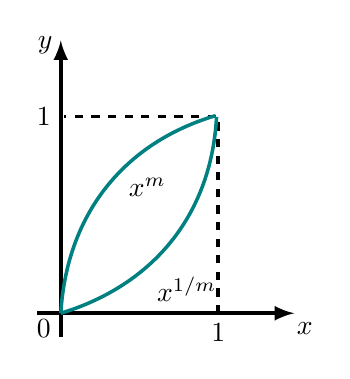
\begin{tikzpicture}[>=latex,shorten >=1pt,auto, semithick,node distance=2.8cm,scale = 1]
\node[] at (-0.2,3.4) {$y$};
\node[left] at (0,2.5) {$1$};
\node[left] at (0,-0.2) {$0$};
\node[below] at (2.0,0) {$1$};
\node[] at (3.1,-0.2) {$x$};
\node[] at (1.60,0.3) {$x^{1/m}$};
\node[] at (1.1,1.6) {$x^{m}$};
\draw[->,line width=0.5mm] (0.0,-0.3) -- (0.0,3.5);
\draw[->,line width=0.5mm] (-0.3,0.0) -- (3.0,0.0);
\draw[-,line width=0.45mm,dashed](2.0,0.0) -- (2.0,2.5) -- (0.0,2.5);
\path[-,line width=0.45mm]
[teal] (0.0,0.0) edge [bend left = 35]  node  {} (2.0,2.52)
[teal] (0.0,0.0) edge [bend right = 35]  node  {} (1.98,2.53);
\end{tikzpicture}

%answer image 3
\begin{tikzpicture}[>=stealth',shorten >=1pt,auto, semithick,node distance=2.8cm]
\node at (-0.2,3.4) {y};
\node at (-0.2,2.5) {1};
\node at (-0.2,-0.2) {0};
\node at (2.0,-0.2) {1};
\node at (3.1,-0.2) {x};
\node at (1.5,0.3) {$x^{1/m}$};
\node at (0.6,1.0) {$x^{m}$};

\draw[->,line width=0.5mm] (0.0,-0.3) -- (0.0,3.5);
\draw[->,line width=0.5mm] (-0.3,0.0) -- (3.0,0.0);
\draw[-,line width=0.5mm,dashed](2.0,0.0) -- (2.0,2.5);
\draw[-,line width=0.5mm,dashed](0.0,2.5) --(2.0,2.5);

\path [-,line width=0.5mm]
[teal] (0.0,0.0) edge [bend right = 15]  node  {} (2.0,2.5)
[teal] (0.0,0.0) edge [bend right = 35]  node  {} (1.98,2.53);
\end{tikzpicture}

%answer image 4
\begin{tikzpicture}[>=stealth',shorten >=1pt,auto, semithick,node distance=2.8cm]
\node at (-0.2,3.4) {y};
\node at (-0.2,2.5) {1};
\node at (-0.2,-0.2) {0};
\node at (2.0,-0.2) {1};
\node at (3.1,-0.2) {x};
\node at (1.2,1.2) {$x^{m}$};
\node at (0.5,2.2) {$x^{1/m}$};

\draw[->,line width=0.5mm] (0.0,-0.3) -- (0.0,3.5);
\draw[->,line width=0.5mm] (-0.3,0.0) -- (3.0,0.0);
\draw[-,line width=0.5mm,dashed](2.0,0.0) -- (2.0,2.5);
\draw[-,line width=0.5mm,dashed](0.0,2.5) --(2.0,2.5);

\path[-,line width=0.5mm]
[teal] (0.0,0.0) edge [bend left = 15]  node  {} (2.0,2.5)
[teal] (0.0,0.0) edge [bend left = 35]  node  {} (2.0,2.52);
\end{tikzpicture}











